% Created by tikzDevice version 0.10.1 on 2020-02-15 16:09:18
% !TEX encoding = UTF-8 Unicode
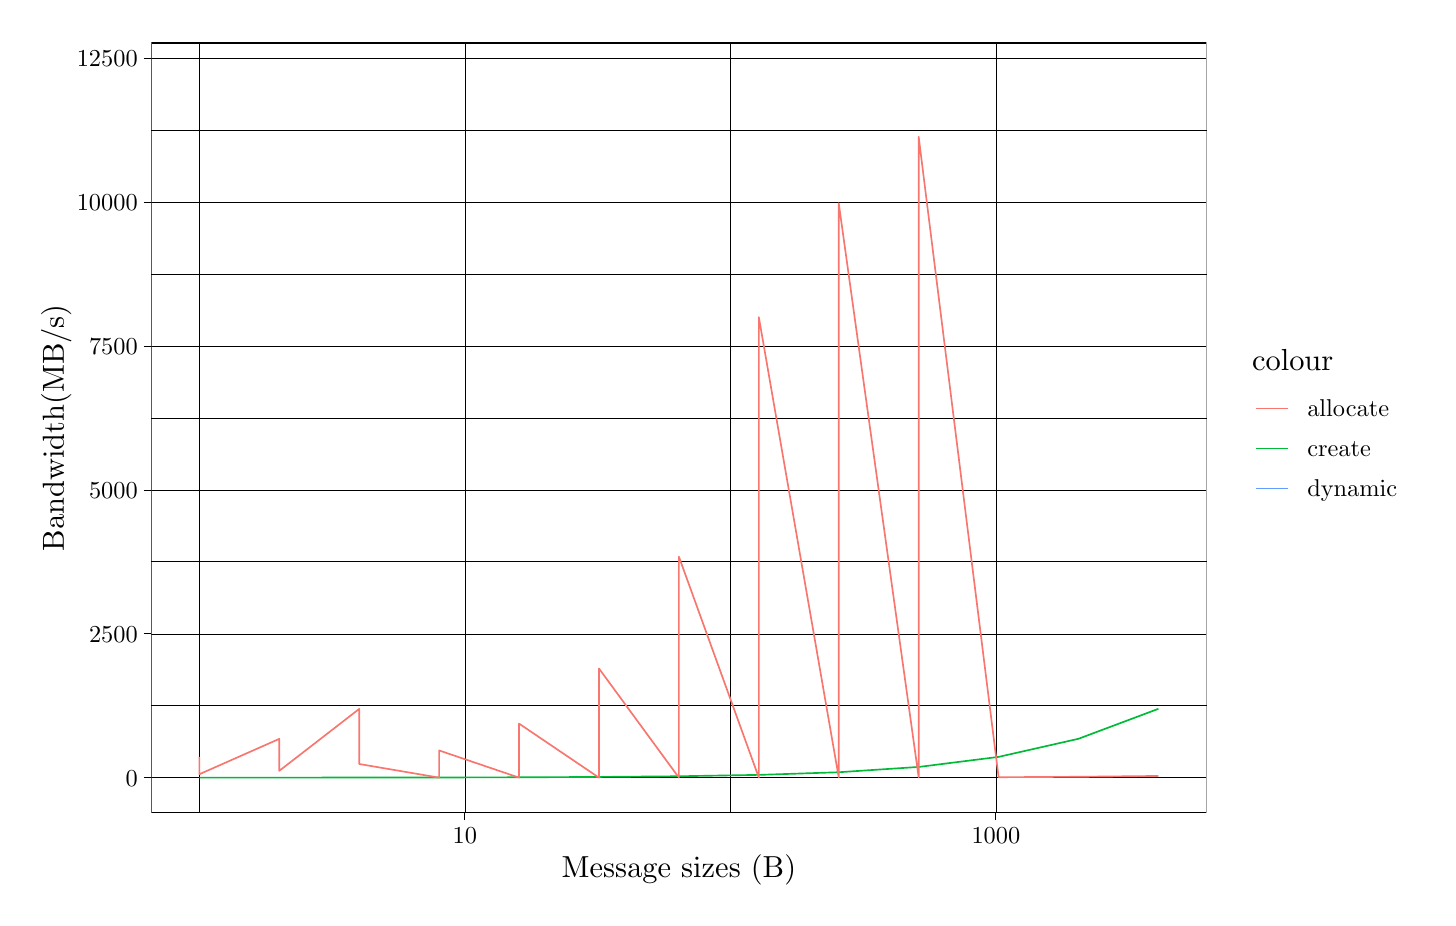
\begin{tikzpicture}[x=1pt,y=1pt]
\definecolor{fillColor}{RGB}{255,255,255}
\path[use as bounding box,fill=fillColor,fill opacity=0.00] (0,0) rectangle (505.89,314.37);
\begin{scope}
\path[clip] (  0.00,  0.00) rectangle (505.89,314.37);
\definecolor{drawColor}{RGB}{255,255,255}
\definecolor{fillColor}{RGB}{255,255,255}

\path[draw=drawColor,line width= 0.6pt,line join=round,line cap=round,fill=fillColor] (  0.00,  0.00) rectangle (505.89,314.37);
\end{scope}
\begin{scope}
\path[clip] ( 44.71, 30.72) rectangle (425.93,308.87);
\definecolor{fillColor}{RGB}{255,255,255}

\path[fill=fillColor] ( 44.71, 30.72) rectangle (425.93,308.87);
\definecolor{drawColor}{RGB}{0,0,0}

\path[draw=drawColor,line width= 0.0pt,line join=round] ( 44.71, 69.35) --
	(425.93, 69.35);

\path[draw=drawColor,line width= 0.0pt,line join=round] ( 44.71,121.33) --
	(425.93,121.33);

\path[draw=drawColor,line width= 0.0pt,line join=round] ( 44.71,173.30) --
	(425.93,173.30);

\path[draw=drawColor,line width= 0.0pt,line join=round] ( 44.71,225.27) --
	(425.93,225.27);

\path[draw=drawColor,line width= 0.0pt,line join=round] ( 44.71,277.25) --
	(425.93,277.25);

\path[draw=drawColor,line width= 0.0pt,line join=round] ( 62.04, 30.72) --
	( 62.04,308.87);

\path[draw=drawColor,line width= 0.0pt,line join=round] (253.92, 30.72) --
	(253.92,308.87);

\path[draw=drawColor,line width= 0.1pt,line join=round] ( 44.71, 43.37) --
	(425.93, 43.37);

\path[draw=drawColor,line width= 0.1pt,line join=round] ( 44.71, 95.34) --
	(425.93, 95.34);

\path[draw=drawColor,line width= 0.1pt,line join=round] ( 44.71,147.31) --
	(425.93,147.31);

\path[draw=drawColor,line width= 0.1pt,line join=round] ( 44.71,199.29) --
	(425.93,199.29);

\path[draw=drawColor,line width= 0.1pt,line join=round] ( 44.71,251.26) --
	(425.93,251.26);

\path[draw=drawColor,line width= 0.1pt,line join=round] ( 44.71,303.23) --
	(425.93,303.23);

\path[draw=drawColor,line width= 0.1pt,line join=round] (157.98, 30.72) --
	(157.98,308.87);

\path[draw=drawColor,line width= 0.1pt,line join=round] (349.86, 30.72) --
	(349.86,308.87);
\definecolor{drawColor}{RGB}{0,186,56}

\path[draw=drawColor,line width= 0.6pt,line join=round] ( 62.04, 43.37) --
	( 62.04, 43.37) --
	( 90.92, 43.38) --
	( 90.92, 43.38) --
	(119.80, 43.40) --
	(119.80, 43.40) --
	(148.68, 43.43) --
	(148.68, 43.43) --
	(177.56, 43.49) --
	(177.56, 43.49) --
	(206.44, 43.62) --
	(206.44, 43.62) --
	(235.32, 43.87) --
	(235.32, 43.87) --
	(264.20, 44.37) --
	(264.20, 44.36) --
	(293.08, 45.32) --
	(293.08, 45.32) --
	(321.96, 47.24) --
	(321.96, 47.23) --
	(350.84, 50.87) --
	(379.72, 57.41) --
	(408.60, 68.24);
\definecolor{drawColor}{RGB}{248,118,109}

\path[draw=drawColor,line width= 0.6pt,line join=round] ( 62.04, 50.84) --
	( 62.04, 44.60) --
	( 90.92, 57.38) --
	( 90.92, 45.83) --
	(119.80, 68.20) --
	(119.80, 48.30) --
	(148.68, 43.37) --
	(148.68, 53.19) --
	(177.56, 43.37) --
	(177.56, 62.89) --
	(206.44, 43.37) --
	(206.44, 82.80) --
	(235.32, 43.38) --
	(235.32,123.21) --
	(264.20, 43.39) --
	(264.20,209.76) --
	(293.08, 43.41) --
	(293.08,250.92) --
	(321.96, 43.44) --
	(321.96,274.93) --
	(350.84, 43.52) --
	(379.72, 43.68) --
	(408.60, 43.98);
\definecolor{drawColor}{RGB}{0,0,0}

\path[draw=drawColor,line width= 0.6pt,line join=round,line cap=round] ( 44.71, 30.72) rectangle (425.93,308.87);
\end{scope}
\begin{scope}
\path[clip] (  0.00,  0.00) rectangle (505.89,314.37);
\definecolor{drawColor}{RGB}{0,0,0}

\node[text=drawColor,anchor=base east,inner sep=0pt, outer sep=0pt, scale=  0.88] at ( 39.76, 40.34) {0};

\node[text=drawColor,anchor=base east,inner sep=0pt, outer sep=0pt, scale=  0.88] at ( 39.76, 92.31) {2500};

\node[text=drawColor,anchor=base east,inner sep=0pt, outer sep=0pt, scale=  0.88] at ( 39.76,144.28) {5000};

\node[text=drawColor,anchor=base east,inner sep=0pt, outer sep=0pt, scale=  0.88] at ( 39.76,196.26) {7500};

\node[text=drawColor,anchor=base east,inner sep=0pt, outer sep=0pt, scale=  0.88] at ( 39.76,248.23) {10000};

\node[text=drawColor,anchor=base east,inner sep=0pt, outer sep=0pt, scale=  0.88] at ( 39.76,300.20) {12500};
\end{scope}
\begin{scope}
\path[clip] (  0.00,  0.00) rectangle (505.89,314.37);
\definecolor{drawColor}{RGB}{0,0,0}

\path[draw=drawColor,line width= 0.3pt,line join=round] ( 41.96, 43.37) --
	( 44.71, 43.37);

\path[draw=drawColor,line width= 0.3pt,line join=round] ( 41.96, 95.34) --
	( 44.71, 95.34);

\path[draw=drawColor,line width= 0.3pt,line join=round] ( 41.96,147.31) --
	( 44.71,147.31);

\path[draw=drawColor,line width= 0.3pt,line join=round] ( 41.96,199.29) --
	( 44.71,199.29);

\path[draw=drawColor,line width= 0.3pt,line join=round] ( 41.96,251.26) --
	( 44.71,251.26);

\path[draw=drawColor,line width= 0.3pt,line join=round] ( 41.96,303.23) --
	( 44.71,303.23);
\end{scope}
\begin{scope}
\path[clip] (  0.00,  0.00) rectangle (505.89,314.37);
\definecolor{drawColor}{RGB}{0,0,0}

\path[draw=drawColor,line width= 0.3pt,line join=round] (157.98, 27.97) --
	(157.98, 30.72);

\path[draw=drawColor,line width= 0.3pt,line join=round] (349.86, 27.97) --
	(349.86, 30.72);
\end{scope}
\begin{scope}
\path[clip] (  0.00,  0.00) rectangle (505.89,314.37);
\definecolor{drawColor}{RGB}{0,0,0}

\node[text=drawColor,anchor=base,inner sep=0pt, outer sep=0pt, scale=  0.88] at (157.98, 19.71) {10};

\node[text=drawColor,anchor=base,inner sep=0pt, outer sep=0pt, scale=  0.88] at (349.86, 19.71) {1000};
\end{scope}
\begin{scope}
\path[clip] (  0.00,  0.00) rectangle (505.89,314.37);
\definecolor{drawColor}{RGB}{0,0,0}

\node[text=drawColor,anchor=base,inner sep=0pt, outer sep=0pt, scale=  1.10] at (235.32,  7.44) {Message sizes (B)};
\end{scope}
\begin{scope}
\path[clip] (  0.00,  0.00) rectangle (505.89,314.37);
\definecolor{drawColor}{RGB}{0,0,0}

\node[text=drawColor,rotate= 90.00,anchor=base,inner sep=0pt, outer sep=0pt, scale=  1.10] at ( 13.08,169.80) {Bandwidth(MB/s)};
\end{scope}
\begin{scope}
\path[clip] (  0.00,  0.00) rectangle (505.89,314.37);
\definecolor{fillColor}{RGB}{255,255,255}

\path[fill=fillColor] (436.93,135.11) rectangle (500.39,204.49);
\end{scope}
\begin{scope}
\path[clip] (  0.00,  0.00) rectangle (505.89,314.37);
\definecolor{drawColor}{RGB}{0,0,0}

\node[text=drawColor,anchor=base west,inner sep=0pt, outer sep=0pt, scale=  1.10] at (442.43,190.44) {colour};
\end{scope}
\begin{scope}
\path[clip] (  0.00,  0.00) rectangle (505.89,314.37);
\definecolor{fillColor}{RGB}{255,255,255}

\path[fill=fillColor] (442.43,169.52) rectangle (456.89,183.97);
\end{scope}
\begin{scope}
\path[clip] (  0.00,  0.00) rectangle (505.89,314.37);
\definecolor{drawColor}{RGB}{248,118,109}

\path[draw=drawColor,line width= 0.6pt,line join=round] (443.88,176.74) -- (455.44,176.74);
\end{scope}
\begin{scope}
\path[clip] (  0.00,  0.00) rectangle (505.89,314.37);
\definecolor{drawColor}{RGB}{248,118,109}

\path[draw=drawColor,line width= 0.6pt,line join=round] (443.88,176.74) -- (455.44,176.74);
\end{scope}
\begin{scope}
\path[clip] (  0.00,  0.00) rectangle (505.89,314.37);
\definecolor{drawColor}{RGB}{248,118,109}

\path[draw=drawColor,line width= 0.6pt,line join=round] (443.88,176.74) -- (455.44,176.74);
\end{scope}
\begin{scope}
\path[clip] (  0.00,  0.00) rectangle (505.89,314.37);
\definecolor{fillColor}{RGB}{255,255,255}

\path[fill=fillColor] (442.43,155.06) rectangle (456.89,169.52);
\end{scope}
\begin{scope}
\path[clip] (  0.00,  0.00) rectangle (505.89,314.37);
\definecolor{drawColor}{RGB}{0,186,56}

\path[draw=drawColor,line width= 0.6pt,line join=round] (443.88,162.29) -- (455.44,162.29);
\end{scope}
\begin{scope}
\path[clip] (  0.00,  0.00) rectangle (505.89,314.37);
\definecolor{drawColor}{RGB}{0,186,56}

\path[draw=drawColor,line width= 0.6pt,line join=round] (443.88,162.29) -- (455.44,162.29);
\end{scope}
\begin{scope}
\path[clip] (  0.00,  0.00) rectangle (505.89,314.37);
\definecolor{drawColor}{RGB}{0,186,56}

\path[draw=drawColor,line width= 0.6pt,line join=round] (443.88,162.29) -- (455.44,162.29);
\end{scope}
\begin{scope}
\path[clip] (  0.00,  0.00) rectangle (505.89,314.37);
\definecolor{fillColor}{RGB}{255,255,255}

\path[fill=fillColor] (442.43,140.61) rectangle (456.89,155.06);
\end{scope}
\begin{scope}
\path[clip] (  0.00,  0.00) rectangle (505.89,314.37);
\definecolor{drawColor}{RGB}{97,156,255}

\path[draw=drawColor,line width= 0.6pt,line join=round] (443.88,147.84) -- (455.44,147.84);
\end{scope}
\begin{scope}
\path[clip] (  0.00,  0.00) rectangle (505.89,314.37);
\definecolor{drawColor}{RGB}{97,156,255}

\path[draw=drawColor,line width= 0.6pt,line join=round] (443.88,147.84) -- (455.44,147.84);
\end{scope}
\begin{scope}
\path[clip] (  0.00,  0.00) rectangle (505.89,314.37);
\definecolor{drawColor}{RGB}{97,156,255}

\path[draw=drawColor,line width= 0.6pt,line join=round] (443.88,147.84) -- (455.44,147.84);
\end{scope}
\begin{scope}
\path[clip] (  0.00,  0.00) rectangle (505.89,314.37);
\definecolor{drawColor}{RGB}{0,0,0}

\node[text=drawColor,anchor=base west,inner sep=0pt, outer sep=0pt, scale=  0.88] at (462.39,173.71) {allocate};
\end{scope}
\begin{scope}
\path[clip] (  0.00,  0.00) rectangle (505.89,314.37);
\definecolor{drawColor}{RGB}{0,0,0}

\node[text=drawColor,anchor=base west,inner sep=0pt, outer sep=0pt, scale=  0.88] at (462.39,159.26) {create};
\end{scope}
\begin{scope}
\path[clip] (  0.00,  0.00) rectangle (505.89,314.37);
\definecolor{drawColor}{RGB}{0,0,0}

\node[text=drawColor,anchor=base west,inner sep=0pt, outer sep=0pt, scale=  0.88] at (462.39,144.81) {dynamic};
\end{scope}
\end{tikzpicture}
